\documentclass{article}
\usepackage[utf8]{inputenc}
%\usepackage[english]{babel}
\usepackage[portuguese]{babel}
\usepackage{graphicx}
\usepackage[hidelinks]{hyperref}
\usepackage{amsmath} %lets us use \begin{proof}
%\usepackage[]{amssymb} %gives us the character \varnothing

\title{Universidade Federal de Pernambuco \\
Macroeconomia 1 - Lista 2}
\author{Monitor: Paulo Francisco (paulfsilva7@gmail.com);}
\date{22 de fevereiro de 2023}


\begin{document}
\maketitle %This command prints the title based on information entered above

%Section and subsection automatically number unless you put the asterisk next to them.
\section*{Questão 1}

\subsection*{Letra A)}
\begin{figure}[!tbh]
    \centering
    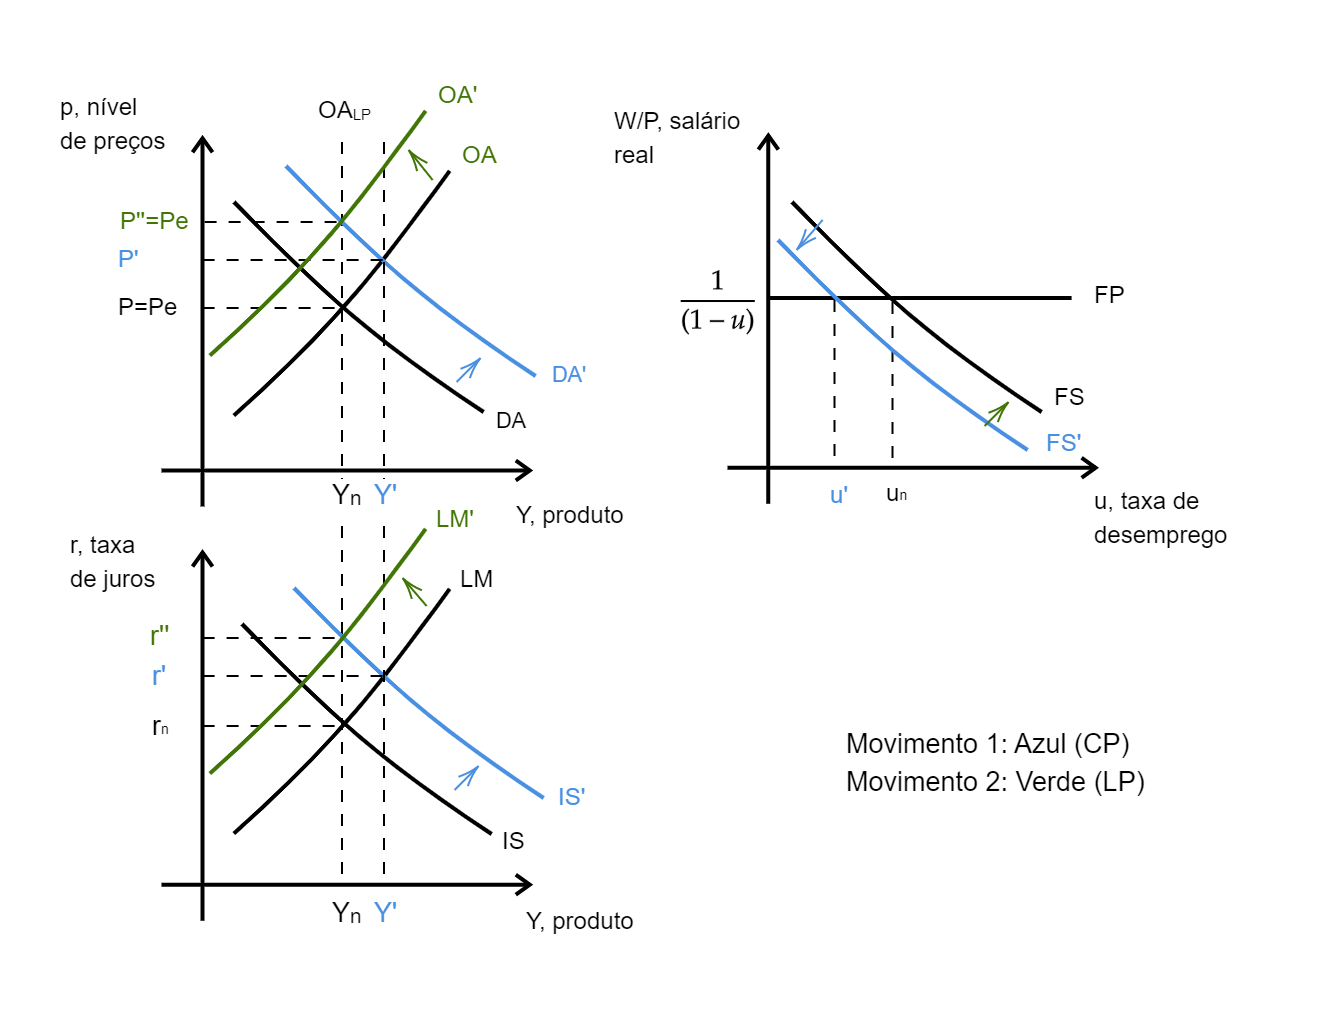
\includegraphics[width=\textwidth]{Grafico - Q1A PNG.png}
    \caption{Aumento do deficit primário}
\end{figure}

O aumento do deficit primário $(G-T)$ resulta na expansão tanto da curva IS quando da curva DA para a direita, aumentando o nível de produto, taxa de juros, nível de preços, e reduzindo o desemprego, na situação de \textbf{curto prazo}.

\textbf{Do curto para o longo prazo}: Com o nível de produção maior que o natural $(Y'>Y_n)$, e um maior nível de preços, os trabalhadores demandarão um salário maior (pelo fato das expectativas estarem desajustadas, isto é, esperavam $P_e=P$, mas preços foram $P'>P_e$. Diante do aumento de $W$ (custo marginal) as firmas, pela regra de fixação de preços (estabelecem preços como um markup sobre o CMg), reajustam preços. O processo de ajuste de expectativas faz com que a OA se desloque para a esquerda (A OA de curto prazo vai cortar a $OA_{LP}$ exatamente no ponto onde $P'=P^\prime_e$. Note que enquanto o produto estiver acima do potencial, $y_n$, as expectativas de preços continuam desajustadas. O processo de ajustamento $\uparrow W \Rightarrow \uparrow P \Rightarrow$ deslocamento da $OA$ para a esquerda continuará até que a economia retorne ao LP. Ao mesmo tempo em que o nível de preços sobe, a razão $\frac{M}{P}$ diminui (se o BC não mexe no M), resultando na contração da oferta de moeda, ou seja, contraindo a curva LM, levando o produto e consequentemente o desemprego de volta para o seu nível natural, no longo prazo. No novo equilíbrio de LP, a economia voltará a exibir o mesmo nível de produto, $Y_n$, e desemprego, $u_n$, mas terá preços maiores $P"$ e juros maiores $r"$.


\subsection*{Letra B)}
\begin{figure}[!tbh]
    \centering
    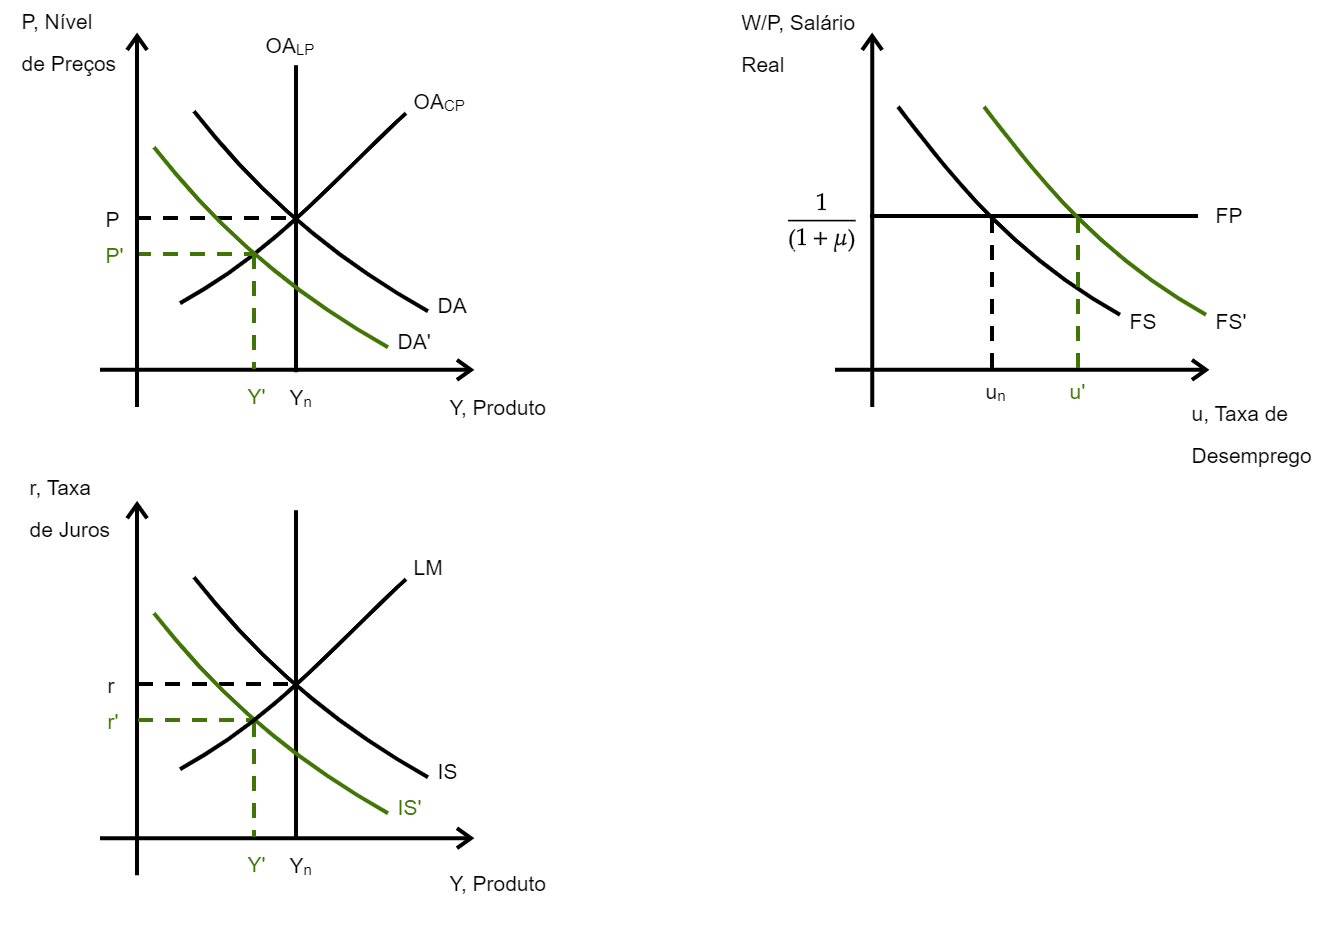
\includegraphics[width=\textwidth]{Q1BCP.png}
    \caption{Expectativas negativas dos investidores}
\end{figure}
\textbf{Curto Prazo:}Um choque de expectativa negativa por parte dos investidores reduz o investimento e consequentemente desloca tanto a curva IS quanto a curva DA para esquerda, produzindo um produto menor no curto prazo. Para um menor nível de produção menos trabalho é requerido de forma que o desemprego aumenta e assim o poder de barganha dos trabalhadores é menor levando-os a aceitar um salário nominal mais baixos diminuindo portanto o salário real, o que consequentemente levará a uma redução no nível de preços da economia de forma que o estoque real de moeda aumenta conduzindo uma menor taxa de juros.

\section*{Questão 2}
\subsection*{Letra A)}
Falso; O aumento do preço esperado retrai a curva de OA, levando para um menor nível de produto e maior nível de preços, enquanto o aumento dos gastos públicos estimularia positivamente a curva DA, aumentando o nível de produto e reduzindo o nível de preços.


\subsection*{Letra B)}
Verdadeiro; A expansão monetária expande a curva DA para a direita, aumentando o nível de preço e produto de curto prazo, mas com os ajustes das expectativas de preço por parte dos agentes a curva OA se retrai levando o produto de volta ao equilíbrio.

\subsection*{Letra C)}
Falso; Uma redução do deficit público $(G-T)$ retrai o produto de equilíbrio.

\subsection*{Letra D)}
Verdadeiro; Com o aumento do preço da matéria-prima o markup das empresas aumentam, $(P-CMg)$, de forma que a curva de fixação de preços cai, levando a um salário nominal mais baixo e um maior nível de desemprego.

\subsection*{Letra E)}
Falso; Um corte de gastos públicos combinado com uma redução de impostos de mesma magnitude terá efeito nulo. $(G-T)=0$

\clearpage %Gives us a page break before the next section. Optional.

\section*{Questão 3}
\subsection*{Letra A)}
$$ C = c_0 + c_1 Y_D - c_2 r; \quad
I = b_0 + b_1 Y_D - b_2 r; \quad G= G_0;$$
$$T=t_0+t_1 Y;\quad \frac{M^{D}}{P} = \frac{M^{S}}{P}; 
\quad \frac{M^{D}}{P} = d_1 Y - d_2 r $$
\\
Para a IS o produto será dado por $Y=C+I+G$:
\begin{equation}
Y = c_0 + c_1 Y_D - c_2 r + b_0 + b_1 Y_D - b_2 r + G_0
\end{equation}

\begin{equation}
Y = c_0 + (c_1+b_1)(Y-t_0-t_1Y) + b_0 - (b_2 +c_2) r + G_0
\end{equation}

\begin{equation}
Y = c_0 + (c_1+b_1)(Y(1-t_1)-t_0) + b_0 - (b_2 +c_2) r + G_0
\end{equation}

\begin{equation}\label{eq:3AY}
Y = c_0 + Y(1-t_1)(c_1+b_1)-t_0(c_1+b_1) + b_0 - (b_2 +c_2) r + G_0
\end{equation}
\begin{equation}
Y[1-(1-t_1)(c_1+b_1)] = c_0-t_0(c_1+b_1) + b_0 - (b_2 +c_2) r + G_0
\end{equation}
\begin{equation}
\textbf{IS:} \>\>\> Y= [c_0-t_0(c_1+b_1) + b_0 - (b_2 +c_2) r + G_0]\frac{1}{1-(1-t_1)(c_1+b_1)}
\end{equation}
\\
Encontrando a LM, sabendo que $\frac{M^S}{P}=\frac{M^D}{P}=\frac{\bar{M}}{P}$:
\begin{equation}
\frac{\bar{M}}{P} = d_1Y-d_2r
\end{equation}

\begin{equation}
d_2r = d_1Y - \frac{\bar{M}}{P}
\end{equation}

\begin{equation}\label{eq:3Ar}
\textbf{LM:} \>\>\> r = \frac{d_1Y}{d_2} - \frac{\bar{M}}{Pd_2}
\end{equation}
\\
Portanto, substituindo \eqref{eq:3Ar} em \eqref{eq:3AY}:

\begin{equation}
Y = c_0 + Y(1-t_1)(c_1+b_1)-t_0(c_1+b_1) + b_0 - (b_2 +c_2)\left[ \frac{d_1Y}{d_2} - \frac{\bar{M}}{Pd_2}\right] + G_0
\end{equation}

\begin{equation}
Y = c_0 + Y(1-t_1)(c_1+b_1)-t_0(c_1+b_1) + b_0 - (b_2 +c_2) \frac{d_1Y}{d_2} + (b_2 +c_2)\frac{\bar{M}}{Pd_2} + G_0
\end{equation}

\begin{equation}
Y = c_0 + Y\left[(1-t_1)(c_1+b_1)-(b_2 +c_2) \frac{d_1}{d_2} \right]-t_0(c_1+b_1) + b_0 + (b_2 +c_2)\frac{\bar{M}}{Pd_2} + G_0
\end{equation}
\\
Mas, isolando Y temos o Y de equilíbrio:
\begin{equation}
Y - Y\left[(1-t_1)(c_1+b_1)-(b_2 +c_2) \frac{d_1}{d_2} \right] = c_0 -t_0(c_1+b_1) + b_0 + (b_2 +c_2)\frac{\bar{M}}{Pd_2} + G_0
\end{equation}

\begin{equation}
Y\left[1-(1-t_1)(c_1+b_1)+(b_2 +c_2) \frac{d_1}{d_2} \right] = c_0 -t_0(c_1+b_1) + b_0 + (b_2 +c_2)\frac{\bar{M}}{Pd_2} + G_0
\end{equation}

\begin{equation}\label{eq:3AYstar}
Y^{*} = \frac{c_0 -t_0(c_1+b_1) + b_0 + (b_2 +c_2)\frac{\bar{M}}{Pd_2} + G_0}{\left[1-(1-t_1)(c_1+b_1)+(b_2 +c_2) \frac{d_1}{d_2} \right]}
\end{equation}
\\
Substituindo a equação \eqref{eq:3AYstar} em \eqref{eq:3Ar}, temos a taxa de juros do equilíbrio:

\begin{equation}\label{eq:3Arstar}
r^{*} = \frac{d_1}{d_2} \frac{c_0 -t_0(c_1+b_1) + b_0 + (b_2 +c_2)\frac{\bar{M}}{Pd_2} + G_0}{\left[1-(1-t_1)(c_1+b_1)+(b_2 +c_2) \frac{d_1}{d_2} \right]} - \frac{\bar{M}}{Pd_2}
\end{equation}

\subsection*{Letra B)}
Sabemos que:

\begin{equation}
    \textit{Fixação de Salários: } W = P^{e}(1 - \alpha u + Z)
    \label{eq:FS}
\end{equation}

\begin{equation}
    \textit{Fixação de Preços: } P=(1+ \mu )W
    \label{eq:FP}
\end{equation}

\begin{itemize}
    \item \begin{text}
            Então substituímos \eqref{eq:FS} em \eqref{eq:FP} para eliminar W:\\
            \begin{equation}
                P=(1+ \mu)P^{e}(1 - \alpha u + Z)
                \label{eq:OAPart1}
            \end{equation}
        \end{text}
    
    \item \begin{text}
            Mas, precisamos achar relação entre P e Y, e sabemos que:\\
            \begin{equation}
                u = \frac{U}{L} = \frac{L-N}{L} = 1 - \frac{Y}{L}
                \label{eq:OAPart2}
            \end{equation}
        \end{text}
        
    \item \begin{text}
            Assim, podemos substituir \eqref{eq:OAPart2} em \eqref{eq:OAPart1}:\\
            \begin{equation}
                P=(1+ \mu)P^{e}\left[1 - \alpha \left(1-\frac{Y}{L} \right) + Z\right]
                \label{eq:OAPart3}
            \end{equation}\\
            Agora temos uma relação entre P e Y, ou seja, derivamos a cuva OA.
        \end{text}
    \item \begin{text}
        Por fim, encontramos o nível de preços de equilíbrio substituindo  o produto de equilíbrio \eqref{eq:3AYstar} na última equação:
        \begin{equation}
            P^*=(1+ \mu)P^{e}\left[1 - \alpha \left(1-\frac{1}{L}\frac{c_0 -t_0(c_1+b_1) + b_0 + (b_2 +c_2)\frac{\bar{M}}{Pd_2} + G_0}{\left[1-(1-t_1)(c_1+b_1)+(b_2 +c_2) \frac{d_1}{d_2} \right]}  \right) + Z\right]
        \end{equation}
    \end{text}
\end{itemize}

\subsection*{Letra C)}
Pela função através da IS:
\begin{equation}
\frac{\partial Y^*}{\partial G} = \frac{1}{\left[1-(1-t_1)(c_1+b_1)+(b_2 +c_2) \frac{d_1}{d_2} \right]} > 0
\end{equation}
\\
Pela função de O.A, derivada na letra B, temos que:
\begin{equation}
\frac{\partial P^*}{\partial Y^*} = \frac{\partial P^*}{\partial Y^*}\frac{\partial Y^*}{\partial G} = \frac{\alpha(1+\mu)P^{e}}{L\left[1-(1-t_1)(c_1+b_1)+(b_2 +c_2) \frac{d_1}{d_2} \right]} > 0
\end{equation}
\\
Para a taxa de juros, encontramos que:
\begin{equation}
\frac{\partial r^*}{\partial G} = \frac{d_1}{d_2} \frac{1}{\left[1-(1-t_1)(c_1+b_1)+(b_2 +c_2) \frac{d_1}{d_2} \right]} > 0
\end{equation}
\\
Como a taxa de desemprego é definida por $u=\left(1-\frac{Y*}{L}\right)$, temos:
\begin{equation}
\frac{\partial u^*}{\partial G}=\frac{\partial u^*}{\partial Y^*}\frac{\partial Y^*}{\partial G}=-\frac{1}{L\left[1-(1-t_1)(c_1+b_1)+(b_2 +c_2) \frac{d_1}{d_2} \right]} <0
\end{equation}
Ou seja, o aumento do gasto do governo induz um aumento na taxa de juros, aumento do produto, eleva o nível de preços, e reduzir a taxa de desemprego.
\clearpage

\subsection*{Letra D)}
\begin{figure}[!tbh]
    \centering
    \includegraphics[width=\textwidth]{Grafico - Q3d PNG.png}
    \caption{Aumento do deficit primário com BC intervindo}
\end{figure}

O aumento dos gastos do governo levaria a um aumento no produto e taxa de juros, mas buscando manter a taxa de juros constante, o BC pode implementar uma politica monetária expansionista de forma que a taxa de juros se mantém constante, porém intensifica os efeitos iniciais do aumento dos gastos do governo, ou seja, causa um aumento do produto, do nível de preços e uma redução da taxa de desemprego ainda maior sobre as variáveis afetadas pelo efeito da política fiscal.

\clearpage
\section*{Questão 4)}
$$C = \bar{C}+c_y Y_D - c_r r^{e}; \hspace{0.5cm} 
I = \bar{I}+i_y Y_D - i_r r^{e}; \hspace{0.5cm}
G = \bar{G}+g_y Y;$$
$$T = \bar{T}+t_y Y; \hspace{0.5cm} 
\frac{M^D}{P} = l_y Y - l_r r; \hspace{0.5cm} 
\frac{M^S}{P}=\frac{\bar{M}}{P}; \hspace{0.5cm} 
r^e=r+s;$$

\subsection*{Letra A)}
Formando a equação da IS, sabendo que $Y=C+I+G$, temos:
\begin{equation}
Y=\bar{C}+c_y Y_D - c_r r^{e} + \bar{I}+i_y Y_D - i_r r^{e} + \bar{G}+g_y Y;
\end{equation}

\begin{equation}
Y=\bar{C}+(c_y+i_y)Y_D - (c_r+i_r)r^{e} + \bar{I} + \bar{G}+g_y Y;
\end{equation}

\begin{equation}
Y=\bar{C}+(c_y+i_y)(Y-\bar{T}-t_yY) - (c_r+i_r)(r+s) + \bar{I} + \bar{G}+g_y Y;
\end{equation}

\begin{equation}\label{eq:4AY}
Y=\bar{C}+Y\left[(1-t_y)(c_y+i_y)+g_y\right]-\bar{T}(c_y+i_y) - (c_r+i_r)(r+s) +\bar{I} +\bar{G};
\end{equation}
\begin{equation}
Y\left[1 -(1-t_y)(c_y+i_y)-g_y\right]=\bar{C}-\bar{T}(c_y+i_y) - (c_r+i_r)(r+s) +\bar{I} +\bar{G};
\end{equation}
\begin{equation}
\textbf{IS:} \>\>\> Y=\frac{\bar{C}-\bar{T}(c_y+i_y) - (c_r+i_r)(r+s) +\bar{I} +\bar{G}}{\left[1 -(1-t_y)(c_y+i_y)-g_y\right]}
\end{equation}
\\
Montando a LM, sabendo que $\frac{M^D}{P}=\frac{M^S}{P}=\frac{\bar{M}}{P}$, teremos:
\begin{equation}
l_r r = l_yY - \frac{M}{P}    
\end{equation}

\begin{equation}\label{eq:4Ar}
\textbf{LM:} \>\>\> r = \frac{l_yY}{l_r} - \frac{\bar{M}}{Pl_r}    
\end{equation}
\\
Substituindo \eqref{eq:4Ar} em \eqref{eq:4AY}, temos o produto de equilíbrio:

\begin{equation}
Y=\bar{C}+Y\left[(1-t_y)(c_y+i_y)+g_y\right]-\bar{T}(c_y+i_y) - r(c_r+i_r)-s(c_r+i_r) +\bar{I} +\bar{G};
\end{equation}

\begin{equation}
Y=\bar{C}+Y\left[(1-t_y)(c_y+i_y)+g_y\right]-\bar{T}(c_y+i_y) - \left(\frac{l_yY}{l_r} - \frac{\bar{M}}{Pl_r}\right)(c_r+i_r)-s(c_r+i_r) +\bar{I} +\bar{G};
\end{equation}

\begin{equation}
Y=\bar{C}+Y\left[(1-t_y)(c_y+i_y)+g_y\right]-\bar{T}(c_y+i_y) - \frac{l_yY}{l_r}(c_r+i_r) + \frac{\bar{M}}{Pl_r}(c_r+i_r)-s(c_r+i_r) +\bar{I} +\bar{G};
\end{equation}

\begin{equation}
Y=\bar{C}+Y\left[(1-t_y)(c_y+i_y)+g_y - \frac{l_y}{l_r}(c_r+i_r)\right]-\bar{T}(c_y+i_y) + \frac{\bar{M}}{Pl_r}(c_r+i_r)-s(c_r+i_r) +\bar{I} +\bar{G};
\end{equation}

\begin{equation}
Y\left[1 - (1-t_y)(c_y+i_y)-g_y+\frac{l_y}{l_r}(c_r+i_r)\right]=\bar{C}-\bar{T}(c_y+i_y) + \frac{\bar{M}}{Pl_r}(c_r+i_r)-s(c_r+i_r) +\bar{I} +\bar{G};
\end{equation}
O produto de equilíbrio portanto será:
\begin{equation}\label{eq:4aystar}
Y^*=\frac{\bar{C}-\bar{T}(c_y+i_y) + \frac{\bar{M}}{Pl_r}(c_r+i_r)-s(c_r+i_r) +\bar{I} +\bar{G}}{\left[1 - (1-t_y)(c_y+i_y)-g_y+\frac{l_y}{l_r}(c_r+i_r)\right]}
\end{equation}
Substituindo portanto na curva LM \eqref{eq:4Ar}, teremos a taxa de juros de equilíbrio:
\begin{equation}\label{eq:4Arstar}
r^* = \frac{l_y}{l_r}\frac{\bar{C}-\bar{T}(c_y+i_y) + \frac{\bar{M}}{Pl_r}(c_r+i_r)-s(c_r+i_r) +\bar{I} +\bar{G}}{\left[1 - (1-t_y)(c_y+i_y)-g_y+\frac{l_y}{l_r}(c_r+i_r)\right]} - \frac{\bar{M}}{Pl_r}   
\end{equation}
\\
O efeito no produto portanto será dado por:
\begin{equation}
    \frac{\partial Y^*}{\partial s} = -\frac{(c_r+i_r)}{\left[1 - (1-t_y)(c_y+i_y)-g_y+\frac{l_y}{l_r}(c_r+i_r)\right]} < 0
\end{equation}
\\
O efeito na taxa de juros portanto será dado por:
\begin{equation}
\frac{\partial r^*}{\partial s} = - \frac{l_y}{l_r}\frac{(c_r+i_r)}{\left[1 - (1-t_y)(c_y+i_y)-g_y+\frac{l_y}{l_r}(c_r+i_r)\right]} < 0 
\end{equation}
Em resumo, o aumento no prêmio de risco reduz tanto a demanda agregada quanto a taxa de juros da economia. Isto é, para um maior prêmio ao risco a taxa de juros e produto de equilíbrio diminuem.

\subsection*{Letra B)}
\begin{figure}[!tbh]
    \centering
    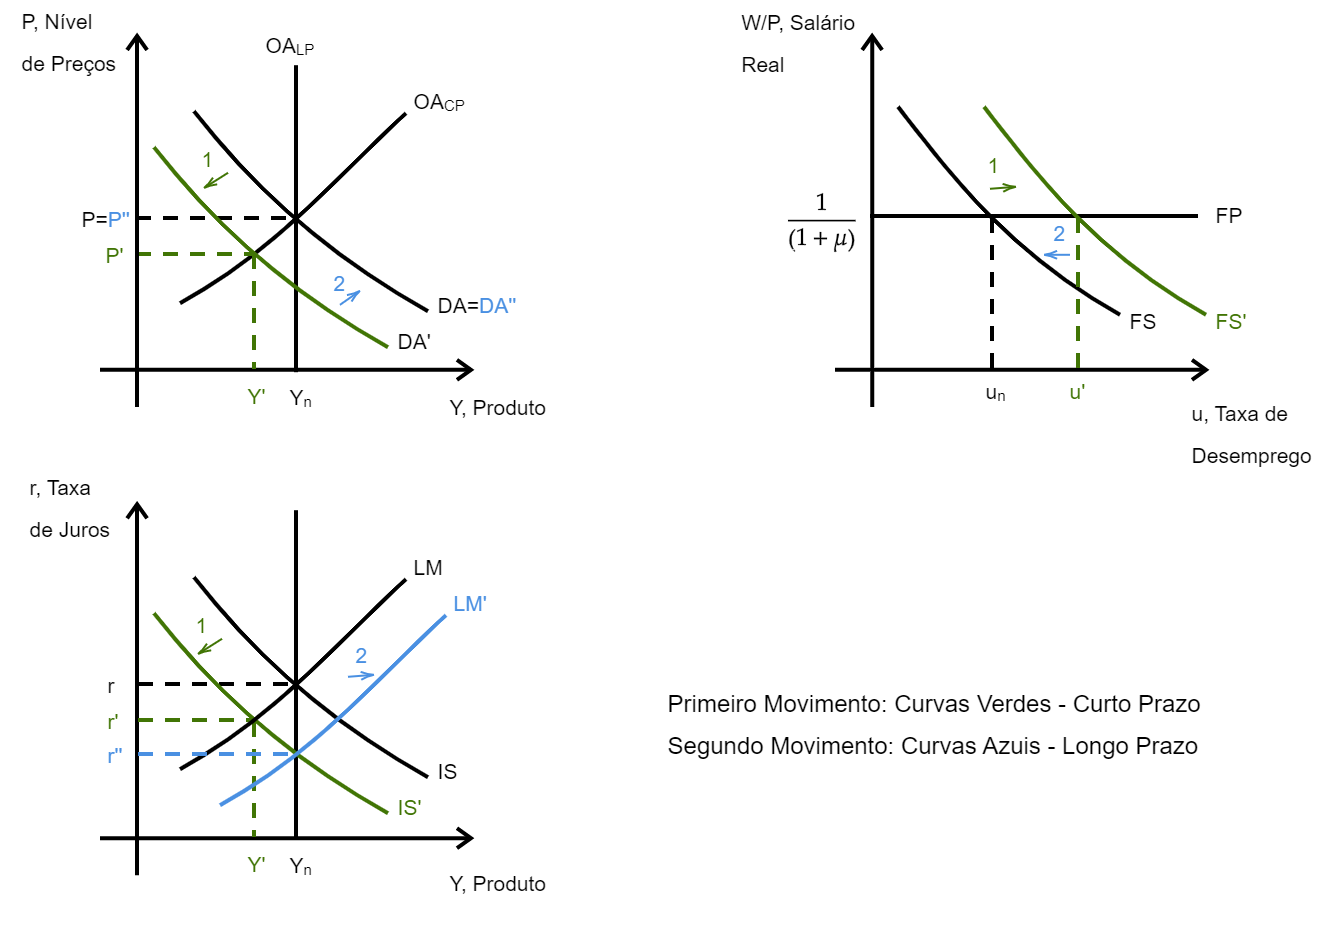
\includegraphics[width=\textwidth]{Q4B.png}
    \caption{Aumento do prêmio ao risco}
\end{figure}
\textbf{Curto Prazo:} Como visto da letra anterior, o aumento do prêmio ao risco reduz consumo e investimento levando a uma queda na renda agregada deslocando tanto a curva IS quanto a curva DA para a esquerda. Com um menor produto de equilíbrio menos trabalho é necessário de forma que o desemprego aumenta, o poder de barganha dos trabalhadores cai fazendo-os aceitar salários nominais mais baixo reduzindo o salário real e induzindo a uma queda dos preços. A queda nos preços aumenta a oferta real de moeda $\frac{M}{P}$ fazendo com que a taxa de juros caia.

\textbf{Longo Prazo:} Preocupado com a estabilidade dos preços, o BC pode expandir a oferta de moeda $M^S$. O aumento da oferta de moeda eleva ainda mais o encaixe real da economia $\frac{M}{P}$ consequentemente reduzindo a taxa de juros e expandindo a curva LM para a direita. Essa política estimula uma maior produção, elevando a demanda agregada para a direita de volta ao nível natural. Com o maior nível de produto mais trabalho se torna necessário e portanto a taxa de emprego aumenta (a taxa de desemprego cai) elevando o salário nominal e o nível de preços até o ponto de volta ao natural.
\end{document}